\documentclass[a4paper,12pt,onside]{scrartcl}
\usepackage[T1]{fontenc}
\usepackage[utf8]{inputenc}
\usepackage{hyperref}
\usepackage{wasysym}% provides \ocircle and \Box
\usepackage{amssymb}
\usepackage{enumitem}% easy control of topsep and leftmargin for lists
\usepackage{color}% used for background color
\usepackage{forloop}% used for \Qrating and \Qlines
\usepackage{ifthen}% used for \Qitem and \QItem
\usepackage{typearea}
\usepackage{tabularx}
\usepackage{tikz}
\usepackage{graphicx}
\usepackage[french]{babel}
%\usepackage{showframe}

%format A4 (21 × 29,7 cm)
\areaset{17cm}{23.7cm}
\usepackage{scrpage2}
\pagestyle{scrheadings}
\ifoot{\today} 
\cfoot{La démarche d’investigation en maternelle}
\ofoot{\pagemark}

%% http://www.svenhartenstein.de/creating-questionnaires-with-latex/

%%%%%%%%%%%%%%%%%%%%%%%%%%%%%%%%%%%%%%%%%%%%%%%%%%%%%%%%%%%%
%% Beginning of questionnaire command definitions %%
%%%%%%%%%%%%%%%%%%%%%%%%%%%%%%%%%%%%%%%%%%%%%%%%%%%%%%%%%%%%
%%
%% 2010, 2012 by Sven Hartenstein
%% mail@svenhartenstein.de
%% http://www.svenhartenstein.de
%%
%% Please be warned that this is NOT a full-featured framework for
%% creating (all sorts of) questionnaires. Rather, it is a small
%% collection of LaTeX commands that I found useful when creating a
%% questionnaire. Feel free to copy and adjust any parts you like.
%% Most probably, you will want to change the commands, so that they
%% fit your taste.
%%
%% Also note that I am not a LaTeX expert! Things can very likely be
%% done much more elegant than I was able to. If you have suggestions
%% about what can be improved please send me an email. I intend to
%% add good tipps to my website and to name contributers of course.
%%
%% 10/2012: Thanks to karathan for the suggestion to put \noindent
%% before \rule!

%% \Qq = Questionaire question. Oh, this is just too simple. It helps
%% making it easy to globally change the appearance of questions.
\newcommand{\Qq}[1]{\textbf{#1}}

%% \QO = Circle or box to be ticked. Used both by direct call and by
%% \Qrating and \Qlist.
\newcommand{\QO}{$\Box$}% or: $\ocircle$

%% \Qrating = Automatically create a rating scale with NUM steps, like
%% this: 0--0--0--0--0.
\newcounter{qr}
\newcommand{\Qrating}[1]{\QO\forloop{qr}{1}{\value{qr} < #1}{---\QO}}

%% \Qline = Again, this is very simple. It helps setting the line
%% thickness globally. Used both by direct call and by \Qlines.
\newcommand{\Qline}[1]{\noindent\rule{#1}{0.6pt}}

%% \Qlines = Insert NUM lines with width=\linewith. You can change the
%% \vskip value to adjust the spacing.
\newcounter{ql}
\newcommand{\Qlines}[1]{\forloop{ql}{0}{\value{ql}<#1}{\vskip0em\Qline{\linewidth}}}

%% \Qlist = This is an environment very similar to itemize but with
%% \QO in front of each list item. Useful for classical multiple
%% choice. Change leftmargin and topsep accourding to your taste.
\newenvironment{Qlist}{%
\renewcommand{\labelitemi}{\QO}
\begin{itemize}[leftmargin=1.5em,topsep=-.5em]
}{%
\end{itemize}
}

%% \Qtab = A "tabulator simulation". The first argument is the
%% distance from the left margin. The second argument is content which
%% is indented within the current row.
\newlength{\qt}
\newcommand{\Qtab}[2]{
\setlength{\qt}{\linewidth}
\addtolength{\qt}{-#1}
\hfill\parbox[t]{\qt}{\raggedright #2}
}

%% \Qitem = Item with automatic numbering. The first optional argument
%% can be used to create sub-items like 2a, 2b, 2c, ... The item
%% number is increased if the first argument is omitted or equals 'a'.
%% You will have to adjust this if you prefer a different numbering
%% scheme. Adjust topsep and leftmargin as needed.
\newcounter{itemnummer}
\newcommand{\Qitem}[2][]{% #1 optional, #2 notwendig
\ifthenelse{\equal{#1}{}}{\stepcounter{itemnummer}}{}
\ifthenelse{\equal{#1}{a}}{\stepcounter{itemnummer}}{}
\begin{enumerate}[topsep=2pt,leftmargin=2.8em]
\item[\textbf{\arabic{itemnummer}#1.}] #2
\end{enumerate}
}

%% \QItem = Like \Qitem but with alternating background color. This
%% might be error prone as I hard-coded some lengths (-5.25pt and
%% -3pt)! I do not yet understand why I need them.
\definecolor{bgodd}{rgb}{0.8,0.8,0.8}
\definecolor{bgeven}{rgb}{0.9,0.9,0.9}
\newcounter{itemoddeven}
\newlength{\gb}
\newcommand{\QItem}[2][]{% #1 optional, #2 notwendig
\setlength{\gb}{\linewidth}
\addtolength{\gb}{-5.25pt}
\ifthenelse{\equal{\value{itemoddeven}}{0}}{%
\noindent\colorbox{bgeven}{\hskip-3pt\begin{minipage}{\gb}\Qitem[#1]{#2}\end{minipage}}%
\stepcounter{itemoddeven}%
}{%
\noindent\colorbox{bgodd}{\hskip-3pt\begin{minipage}{\gb}\Qitem[#1]{#2}\end{minipage}}%
\setcounter{itemoddeven}{0}%
}
}

%%%%%%%%%%%%%%%%%%%%%%%%%%%%%%%%%%%%%%%%%%%%%%%%%%%%%%%%%%%%
%% End of questionnaire command definitions %%
%%%%%%%%%%%%%%%%%%%%%%%%%%%%%%%%%%%%%%%%%%%%%%%%%%%%%%%%%%%%

\renewcommand{\QO}{$\ocircle$}% Use circles now instead of boxes.


%http://tex.stackexchange.com/questions/138968/how-can-i-create-a-brace-spanning-multiple-lines-on-the-right-side-of-an-itemize

\usetikzlibrary{decorations.pathreplacing,calc}

\newcounter{itemnum}

\newcommand{\nt}[2][0pt]{%
    \stepcounter{itemnum}%
    \if###2##%
    \else
        #2%
        \thinspace
    \fi
    \tikz[overlay,remember picture,baseline=(\theitemnum.base),xshift=#1]\node (\theitemnum){};%
}

\newcommand{\makebrace}[4][0pt]{%
    \begin{tikzpicture}[overlay, remember picture]
        \draw [decoration={brace,amplitude=0.5em},decorate]
        let \p1=(#2), \p2=(#3) in
        ({max(\x1+#1,\x2+#1)}, {\y1+1.75ex}) -- 
            node[right=0.6em] {#4} ({max(\x1+#1,\x2+#1)}, {\y2-0.5ex});
    \end{tikzpicture}%
}

\newenvironment{braceitems}{%
    \begin{enumerate}
}{%
    \end{enumerate}
    \setcounter{itemnum}{0}%
}

\newcommand{\fin}{Merci de votre participation, c’est la fin du questionnaire.}

\begin{document}
\begin{center}
	\textbf{\LARGE La démarche d’investigation en maternelle}
\end{center}

Dans le cadre du master Métiers de l’enseignement, de l’éducation et de la formation (Aix-Marseille Université), je rédige un mémoire professionnel ayant pour objectif de savoir comment est mise en œuvre la démarche d’investigation en maternelle. Ce questionnaire contient au maximum 23~questions et une zone de commentaire. 

%\hfill A.~Pachot


\section{Population cible}
\QItem{
	\Qq{Êtes-vous enseignante ou enseignant en maternelle dans une école appliquant les programmes du ministère français de l’Éducation nationale ?}
	\begin{Qlist}
		\item Oui.
		\item Non. $\Rightarrow$ \fin
	\end{Qlist}
}


\section{Cadre}
\QItem{
	\Qq{En quelle section enseignez-vous ?}
	\begin{Qlist}
		\item Grande section.
		\item Moyenne section.
		\item Petite section.
		\item Toute petite section.
	\end{Qlist}
}

\QItem{
	\Qq{À combien de classes enseignez-vous ?}
	\begin{Qlist}
		\item Une seule classe dont je suis la seule enseignante, le seul enseignant.
		\item Une seule classe dont je suis l’enseignante principale, l’enseignant principal.
		\item Une seule classe dont j’enseigne à mi-temps (stagiaire, \dots).
		\item Plusieurs classes dont je suis la modulatrice, le modulateur.
		\item Plusieurs classes dont je suis une remplaçante, un remplaçant.
		\item Autre cas (précisez) : \Qline{4.4in}
	\end{Qlist}
}

\QItem{
	\Qq{Enseignez-vous seulement en maternelle ?}
	\begin{Qlist}
		\item Oui.
		\item Non.
	\end{Qlist}
}

\QItem{
	\Qq{Depuis combien d’années enseignez-vous en maternelle ?}
	\begin{Qlist}
		\item Plus de 10 ans.
		\item Entre 5 et 10 ans.
		\item Moins de 5 ans.
		\item Ne se prononce pas.
	\end{Qlist}
}


\section{Programmes}\label{programmes}
\QItem{
	\Qq{À votre avis, dans les \textit{programmes de 2008}, à partir de quel cycle la démarche d’investigation est-elle explicitement mentionnée pour l’enseignement des sciences ?}
	\begin{Qlist}
		\item Cycle 1.
		\item Cycle 2.
		\item Cycle 3.
		\item Pas d’opinion.
		\item Ne se prononce pas.
	\end{Qlist}
}

\QItem{
	\Qq{À votre avis, dans le \textit{nouveau programme de la maternelle} et les \textit{projets de programme de l’élémentaire}, à partir de quel cycle la démarche d’investigation est-elle explicitement mentionnée pour l’enseignement des sciences ?}
	\begin{Qlist}
		\item Cycle 1 (programme pour la rentrée scolaire 2015).
		\item Cycle 2 (projet de programme pour la rentrée scolaire 2016).
		\item Cycle 3 (projet de programme pour la rentrée scolaire 2016).
		\item Pas d’opinion.
		\item Ne se prononce pas.
	\end{Qlist}
}


\section{Enseignement des sciences}
\QItem{
	\Qq{Laquelle de ces affirmations vous décrit le mieux ?}
	\begin{Qlist}
		\item Je suis une personne très engagée dans l’enseignement des sciences.
		\item Je suis une personne engagée dans l’enseignement des sciences.
		\item Je suis une personne peu engagée dans l’enseignement des sciences.
		\item Je suis une personne pas du tout engagée dans l’enseignement des sciences.
	\end{Qlist}
}

\QItem{
	\Qq{Êtes-vous d’accord avec l’affirmation suivante : \og N’importe quel concept scientifique peut être abordé avec chaque enfant, à n’importe quel âge, à partir de situations adaptées. \fg}
	\begin{Qlist}
		\item Totalement d’accord.
		\item Plutôt d’accord.
		\item Plutôt en désaccord.
		\item Totalement en désaccord.
		\item Pas d’opinion.
		\item Ne se prononce pas.
	\end{Qlist}
}

\QItem{
	\Qq{Êtes-vous d’accord avec l’affirmation suivante : \og Il est possible d’enseigner les sciences en maternelle en utilisant la démarche d’investigation. \fg}
	\begin{Qlist}
		\item Totalement d’accord.
		\item Plutôt d’accord.
		\item Plutôt en désaccord.
		\item Totalement en désaccord.
		\item Pas d’opinion.
		\item Ne se prononce pas.
	\end{Qlist}
}

\QItem{
	\Qq{Enseignez-vous les sciences ?}
	\begin{Qlist}
		\item \nt{Oui.}
		\item \nt{Non, c’est l’autre enseignante qui s’en charge.}
		\item \nt{Non, les sciences ne sont pas enseignées.}
	\end{Qlist}
%	\makebrace{2}{3}{$\Rightarrow$ \begin{minipage}[l]{30ex} \fin \end{minipage}}
	\makebrace{2}{3}{$\Rightarrow$ \begin{minipage}[l]{30ex} Le questionnaire est finie, vous pouvez allez à la fin, aux commentaires (section 7). \end{minipage}}
}

\QItem{
	\Qq{Soit $x$ votre durée moyenne hebdomadaire d’enseignement des sciences en maternelle en heure(s), alors\dots}
	\begin{Qlist}
		\item $x < 1$
		\item $1\leqslant x<2$
		\item $2\leqslant x <3$
		\item $3\leqslant x<4$
		\item $x\geqslant 4$
		\item Ne sait pas.
		\item Ne se prononce pas.
	\end{Qlist}
}


\section{Démarches}
\QItem{
	\Qq{Faites-vous des apports théoriques avant les expériences ?}
	\begin{Qlist}
		\item Toujours.
		\item Souvent.
		\item Occasionnellement.
		\item Jamais.
		\item Ne se prononce pas.
	\end{Qlist}
}

\QItem{
	\Qq{Faites-vous des expériences sans questionnement initial ?}
	\begin{Qlist}
		\item Toujours.
		\item Souvent.
		\item Occasionnellement.
		\item Jamais.
		\item Ne se prononce pas.
	\end{Qlist}
}

\QItem{
	\Qq{Faites-vous des activités exclusivement technologiques, c’est-à-dire de réaliser un objet sans autre problématique.}
	\begin{Qlist}
		\item Toujours.
		\item Souvent.
		\item Occasionnellement.
		\item Jamais.
		\item Ne se prononce pas.
	\end{Qlist}
}


\QItem{
	\Qq{La figure~\ref{demarcheInvestigation} (p.~\pageref{demarcheInvestigation}) est une représentation de la démarche d’investigation. Adoptez-vous la démarche d’investigation lors de vos séances de sciences ?}
	\begin{Qlist}
		\item Toujours.
		\item Souvent.
		\item Occasionnellement.
		\item Jamais.
		\item Ne se prononce pas.
	\end{Qlist}
}
\begin{figure}[h!tbp]
  \centering
  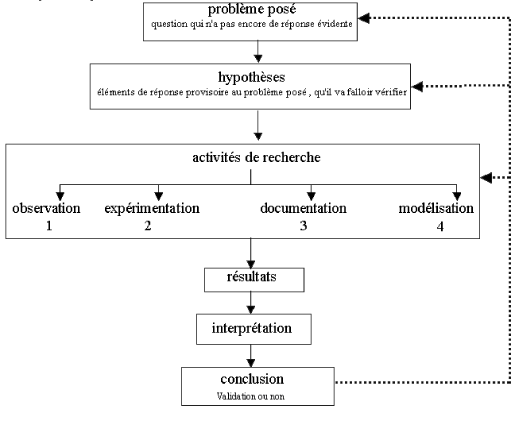
\includegraphics[width=.98\textwidth]{../images/demarcheInvestigation.png}
  \caption{La démarche d’investigation (d’après Dominique Rojat, IGEN SVT)}
  \label{demarcheInvestigation}
\end{figure}

\QItem{
	\Qq{Privilégiez-vous la démarche d’investigation à l’acquisition des connaissances ?}
	\begin{Qlist}
		\item Toujours.
		\item Souvent.
		\item Occasionnellement.
		\item Jamais.
		\item Ne se prononce pas.
	\end{Qlist}
}

\QItem{
	\Qq{Adaptez-vous la démarche d’investigation en formulant vous-même la question problématique plutôt que de construire progressivement en classe le problème à partir d’un étonnement, d’une curiosité ou d’un questionnement ?}
	\begin{Qlist}
		\item Toujours.
		\item Souvent.
		\item Occasionnellement.
		\item Jamais.
		\item Ne se prononce pas.
	\end{Qlist}
}


%\newpage
\section{Lorsque vous utilisez la démarche d’investigation, les activités de recherche réalisées par les élèves s’appuient sur\dots}
\QItem{
	\Qq{\dots{} un dispositif où un seul facteur varie et où les résultats sont recueillis par l’observation ou la mesure (expérimentation directe) :}
	\begin{Qlist}
		\item Toujours.
		\item Souvent.
		\item Occasionnellement.
		\item Jamais.
		\item Ne se prononce pas.
	\end{Qlist}
}

\QItem{
	\Qq{\dots{} divers essais dont les résultats sont comparés (tâtonnement expérimental) :}
	\begin{Qlist}
		\item Toujours.
		\item Souvent.
		\item Occasionnellement.
		\item Jamais.
		\item Ne se prononce pas.
	\end{Qlist}
}

\QItem{
	\Qq{\dots{} une réalisation matérielle (construction d’un objet, d’un modèle, recherche d’une solution technique) :}
	\begin{Qlist}
		\item Toujours.
		\item Souvent.
		\item Occasionnellement.
		\item Jamais.
		\item Ne se prononce pas.
	\end{Qlist}
}

\QItem{
	\Qq{\dots{} une observation directe ou assistée par un instrument (qui ne soit pas l’ordinateur) ou sur l’exploitation de documents (images, données, résultats d’expériences) :}
	\begin{Qlist}
		\item Toujours.
		\item Souvent.
		\item Occasionnellement.
		\item Jamais.
		\item Ne se prononce pas.
	\end{Qlist}
}

\QItem{
	\Qq{\dots{} la lecture de documents papier ou électronique ou par l’interview de personnes compétentes (recherche documentaire) :}
	\begin{Qlist}
		\item Toujours.
		\item Souvent.
		\item Occasionnellement.
		\item Jamais.
		\item Ne se prononce pas.
	\end{Qlist}
}

\section{Commentaires}
\QItem{
	\Qq{Si vous avez des commentaires à ajouter\dots}
	\Qlines{10}
}

\vspace{1em}
\noindent\fin{} Le mémoire sera disponible sur le site suivant: \url{https://github.com/LibreEdu/ESPE/tree/master/UE45_memoire}. Vous pouvez également me le demander en envoyant un courriel à \href{mailto:alexandre.pachot@etu.univ-amu.fr}{\texttt{alexandre.pachot@etu.univ-amu.fr}}.
\end{document}

https://github.com/LibreEdu/ESPE/blob/master/UE45_memoire/memoire_versionNumerique.pdf
http://www.fondation-lamap.org/fr/topic/15107
http://eduscol.education.fr/cid46578/reperes-pour-la-mise-en-oeuvre-d-une-demarche-%C2%A0du-questionnement-a-la-connaissance-en-passant-par-l-experience%C2%A0.html
http://www.ia44.ac-nantes.fr/vie-pedagogique/les-domaines-d-apprentissage-du-premier-degre/culture-scientifique/lettres-des-sciences/lettre-des-sciences-n-3-la-demarche-d-investigation-833751.kjsp
